\chapter{Modelling a Database for Dynamic Multimedia Data}
\label{chapter:system_model}

We have elaborated in \Cref{chapter:applications} that multimedia retrieval and analytics workloads (and workloads that exhibit similiar characteristics) pose specific requirements on a database system. In this chapter, we focus on four aspects and derive a formal model to accomodate them on a system level:

\begin{description}
    \item[Support for Non-atomic Data] Multimedia workloads process features, which are usually real-valued, high-dimensional vectors but can theoretically be any mathematical object (e.g., complex numbers, matrices etc.). A multimedia \acrshort{dbms} must support these objects as first-class citizens.
    \item[Support for Distance Computation] The notion of proximity between features plays a crucial role in all types of multimedia workloads, be it for simple \acrshort{nns} or clustering. While certain workloads rely on raw speed for simple computations and data structures that allow for this type of lookup, other workloads require the ability to compose more complex computations and execute them efficiently without the use of an index. Both aspects must be covered by a multimedia \acrshort{dbms}.
    \item[Dynamically Changing Data] Data is usually subject to constant change and a multimedia \acrshort{dbms} must be able to propagate these changes to all the relevant data structures while maintaining ther internal consistency model.
    \item[Accuracy vs. Time] Multimedia queries often trade retrieval accuracy against speed or vice-versa, e.g., when using a high-dimensional indexes. The multimedia \acrshort{dbms} must allow the user to express their perference at different levels of the system.
\end{description}

To address these requirements, we propose and formalize a set of functionality, which will be specified in the next sections. First, we propose a notion of \emph{generalized, proximity based queries} as an extension to the relational model. Second, we describe a \emph{cost-model} that takes the notion of accuracy of results into acount. And finally, we introduce a general-purpose mechanism to enable high-dimensional indexes to cope with changing data.

All these contributions can be seen as extensions to the functionality provided by a traditional \acrshort{dbms}. To establish a frame of reference, we assume the relational model and \acrshort{acid} properties for the model \acrshort{dbms} under consideration, without a loss of generality.

\section{Generalized Proximity Based Operations}

Starting with the vector space model for similarity search~\cite{Zezula:2006Similarity} presented in \Cref{chapter:theory_multimedia_analysis_and_retrieval}, we propose to extend the notion of distance-based similarity search to that of a more general \emph{proximity based query} following \cref{definition:pbq}.

\begin{definition}[label=definition:pbq]{Proximity Based Query}{}
    Let $\relation$ be a relation. Any database query that relies on the evaluation of a distance function $\delta: \domain_{f} \times \domain_{f} \rightarrow \symreal_{\geq 0}$ that calculates the distance between an attribute $\attribute_{f} \in \schema(\relation)$ and some query $q \in \domain_f$, is called a \emph{proximity based query}. We call $q$ the \emph{query} and $\attribute_{f}$ the \emph{probing argument}, which both share the same \emph{query data domain} $\domain_f$. It is to be noted, that $\domain_f \equiv \symfeatures$. 
\end{definition}

\cref{definition:pbq} simply requires a notion of proximity between some attribute and a query to be obtained by evaluating some distance function. The definition does not make any assumption as to what data domains $\domain_f$ query and probing attribute belong to nor how the distance is being used within the query. 

It is obvious, that similarity search falls into the broader category of a proximity based query, wherein the distance is used to rank a relation and subsequently limit its cardinality. In addition to this common application, the definition of proximity based queries also includes operations such as evaluating a distance function followed by some filtering (e.g., range search) or aggregation based on the computed value (e.g., clustering). That is, we are not limited to mere \acrshort{nns}, since we consider obtaining the distance as one step, which can be freely combined with all other operations supported by the underlying algebra.

\subsection{Revisiting Distance Computation}

Since the choice of the distance function $\symdist$ is a crucial part of any proximity based query, it is worth revisiting its definition. Again, starting with the metric space modell~\cite{Zezula:2006Similarity}, we identify the following (implicit) constraints with respect to the distance function:

\begin{enumerate}
    \item The domain (i.e., the input) of the distance function $\symdist$ is assumed to be $\symreal^{\mathtt{dim}} \times \symreal^{\mathtt{dim}}$, that is, the distance function is assumed to be a binary function and arguments are restricted to real-valued vectors.
    \item The codomain (i.e., the output) of the distance function $\symdist$ is assumed to be $\symreal_{\geq 0}$, hence, the generated distance value is a positive, real number.
    \item The pair $(\domain_f,\symdist)$ usually constitutes a metric, thus satisfying the non-negativity, identity of indiscernibles, symmetry and subadditivity properties.
\end{enumerate}

Upon closer examination and if we consider the use cases presented in \Cref{chapter:applications}, one must come to challenge some of these constraints. If, for example, we turn to \cref{example:mrf}, we realise that it is not reasonable to impose a general restriction of the domain of the distance function to $\symreal^{\mathtt{dim}}$ with $\mathtt{dim} \in \symnatural^{+}$

\begin{example}[label=example:mrf]{\acrlong{mips}{} for \acrshort{mrf}}{}
    In \acrshort{mrf} (see \cref{section:application_mrf}), we try to obtain the signal vector $a_{i \in \mathbb{N}} \in \domain_f \subset \symcomplex^{\mathtt{dim}}$ so that it maximizes the inner product to a signal (query) vector $q \in \symcomplex^{\mathtt{dim}}$. In this case, the distance function $\symdist$ has the form $\symdist \colon \symcomplex^{\mathtt{dim}} \times \symcomplex^{\mathtt{dim}} \to \symreal_{\geq 0}$. Hence, the domain of $\symdist$ is a complex vector space.
\end{example}

Obviously, this limitation of the definition of $\symdist$ can be easily remediated simply by extending the set of supported data domains $\domainset$ by $\symcomplex^{\mathtt{dim}}$ similarily to how it was done for $\symreal^{\mathtt{dim}}$ as proposed by \cite{Giangreco:2018Database}. Nevertheless, we have to acknowledge, that the text-book definition of a distance function is obviously too limited for some real-world applications, and that the query and probing arguments of a distance function could be any type of value supported by the \acrshort{dbms}. Another, similar example could be the \emph{Levenshtein distance}~\cite{Levensthtein:1965Binary} -- often used in computer linguistics -- which is a distance metric on string values.

If now in addition, we consider \cref{example:svmdistance}, we see that restricting oneself to binary functions with $\symreal_{\geq 0}$ is also too limiting when facing certain practical scenarios.

\begin{example}[label=example:svmdistance]{Distance Between a Vector and a Hyperplane}{}
    To find positive and negative examples $a_{i} \in \domain_f \subset \symreal^{\mathtt{dim}}$ given a linear classifier, e.g., provided by a SVM, we evaluate the distances between the attributes and a (query-)hyperplane described as $\mathbf{q}^T\mathbf{x} - b = 0$ with $\mathbf{q},\mathbf{x} \in \symreal^{\mathtt{dim}}$ and $b \in \symreal$. The distance function is then given by:

    \begin{equation}
        \symdist (\mathbf{a}_i, \mathbf{q}, b) = \frac{\left\|\mathbf{q}^T \mathbf{a_i} + b \right\|}{\left\|\mathbf{q}\right\|}
    \end{equation}
    
    $\symdist$ now has the form $\symdist \colon \symreal^{\mathtt{dim}} \times \symreal^{\mathtt{dim}} \times \symreal \to \symreal$. Hence, $\symdist$ is no longer a binary but a ternay function with arguments $\mathbf{a_{i}}$, $\mathbf{q}$ and $b$. Furthermore, the distance may take negative values depending on whether a result is considered a positive or negative example.
\end{example}


Again, we are confronted with an example that violates the text-book definition of a distance function. While the idealized idea that distance functions used in proximity based queries must always constitute a metric on some real-valued vector space may be very common~\cite{Zezula:2006Similarity}, we see in practice that this assumption is often violated~\cite{Skopal:2011Nonmetric,Bernhauer:2019Nonmetric} and that many functions used to calculate proximity between objects are not actual metrics. Even though, this can be a disadvantage when considering high-dimensional index structures that exploit the geometric properties of metric spaces, it is obvious that such functions exist and must thus be considered in any generalised multimedia database application supporting proximity based queries. 

In contrast, there is actually good reason to assume the codomain of a distance function  $\symdist$ to lie in $\symreal$. On the one hand, it is obviously convenient both for the underlying mathematics as well as from an implementation prespective. More importantly, however, real numbers -- unlike, for example, complex numbers or vectors -- come with a natural, total ordering, which is required for downstream operations such as sorting, ranking or clustering.

To summarize, we have established that, on the one hand, we require a proper definition of what is considered to be a valid distance function so as to be able to efficiently plan and execute queries that use them, while on the other hand we must keep that definition open enough to accomodate the many different, applications.

To address the aforementioned limitations while still accomodating classical, metric distances, we propose the extension of a the distance function to the more general notion of a \acrfull{dfc} following \cref{definition:dfc}.

\begin{definition}[label=definition:dfc]{\acrlong{dfc}}{}
    A \acrshort{dfc} $\symdfc \colon \domain_f \times \domain_f \times \domain_{1} \ldots \times \domain_{N} \to \symreal$ is an N-ary but at least binary function $\symdfc(p,q,s_1,\ldots,s_n)$ that outputs a distance $d \in \symreal$ between a probing argument $p \in \domain_f$ and a query argument $q \in \domain_f$ using a defined number of \emph{support arguments} $s_{k \in \mathbb{N}}$ from any of the data domains in $\domainset$.

    As a convention for notation, the probing argument $p$ of a DFC $\symdfc(p,q,s_1,...,s_n)$ will always come first, followed by the query argument $q$, again followed by its support arguments $s_k$ in no particular order.
\end{definition}

\begin{example}[label=example:dfc]{Examples of \acrlong{dfc}es}{}

    A merely illustrative yet widely used example of a \acrshort{dfc} would be the family of \emph{Minkowski Distances} $\symdfc_{M} \colon \symreal^{\mathtt{dim}} \times \symreal^{\mathtt{dim}} \times \symreal \to \symreal_{\geq 0}$. In this context, support argument $m$ is used to convert the higher-order function to a classical distance function, such as, the Manhattan ($L_1$) or Euclidean ($L_2$) distance:

    \begin{equation}
        \symdfc_{M}(\mathbf{p},\mathbf{q},m) = \left(\sum_{i=1}^{n} \mid p_i - q_i \mid^m\right)^{\frac{1}{m}}
    \end{equation}
    
    \begin{equation}
       \symdist_{L1}(\mathbf{p},\mathbf{q}) = \symdfc_M(\mathbf{p},\mathbf{q}, 1) = \sum_{i=1}^{n} \mid p_i - q_i \mid
    \end{equation}
    
    \begin{equation}
       \symdist_{L2}(\mathbf{p},\mathbf{q}) =\symdfc_M(\mathbf{p},\mathbf{q}, 2) = \sqrt{\sum_{i=1}^{n} \mid p_i - q_i \mid^2}
    \end{equation}
    
    However, using the idea of a \acrshort{dfc}, we can express many different types of much more complex distance functions in a simple yet powerful framework. For example, the following distance function is used to obtain a dissimilarity between poses using the joint locations of an 18-keypoint skeleton (details presented in \cite{Heller:2022Multi}):

    \begin{equation}
        \hat{\delta}(\mathbf{p},\mathbf{q},\mathbf{w}_q,\mathbf{w}_f, s) = \sum_{i=1}^{n} \mid (p_i - q_i) \mid \min(w_{q,i}, w_{f,i}) + 2\pi (s - \sum_{i=1}^{n} \min(w_{q,i}, w_{f,i}))
    \end{equation}

    The query and support arguments $\mathbf{p}$ and $\mathbf{q}$ are the actual, normalised keypoints and are accompanied by two weight-vectors $\mathbf{w}_q$ and $\mathbf{w}_f$, that encode the presence or absence of a joint in a scene. To normalise for missing joints, a normalisation factor based on the weight-sum $s$ is employed.

\end{example}


A \acrshort{dfc} (and any function for that matter) is uniquely defined by its \emph{signature}, a ($N+1$)-tuple specifying the name of the \acrshort{dfc} and the data domains $\domain_i$ of the arguments it can accept as defined in \cref{equation:dfc_signature}.

\begin{equation}
    \label{equation:dfc_signature}
    \texttt{SIG}(\symdfc) = (\mathtt{NAME}, \domain_f, \domain_f, \domain_1,... \domain_{N-2})
\end{equation}

In the context a concrete execution plan for a proximity based query, we observe the query argument effectively remains constant, while the probing argument changes as tuples are being evaluated. The support arguments may or may not be subject to change. For example, for simple \acrshort{nns}, there is a single, constant query vector that is compared against all the vectors in the \acrshort{dbms}, i.e., the probing argument. Hence, irrespective of the arity of the \acrshort{dfc}, the function used during query execution comes with an arity of at most $N-1$. We call this the \emph{implementation} of $\symdfc$ as denoted by \cref{equation:dfc_implementation}.

\begin{equation}
    \label{equation:dfc_implementation}
    \symdist = \texttt{IMP}(\symdfc) \ni \texttt{SIG}(\symdist) \subset \texttt{SIG}(\symdfc)
\end{equation}

With this idea of a \acrshort{dfc} and its (partial) implementations in mind, we can start to reason about their properties in the broader context of database operations in general and proximity based queries in particular:

\begin{description}
    \item[\acrshort{dfc} and Proximity Based Queries] In extension to \cref{definition:pbq}, we realise that any query execution plan that involves the evaluation of a (partial) implementation of a \acrshort{dfc}, falls into the category of a proximity based query.

    \item[Variable and Constant Arguments] In the context of a proximity based query, every attribute of a \acrshort{dfc} can either be regarded as \emph{constant} or \emph{variable}. That is, as elements in the database are iterated during query execution, they either remain the same or assume new values. 
    
    \item[Purity of Domain] Since the purpose of a \acrshort{dfc} is to quantify proximity between a probing argument $p$ and a query argument $q$, we can assume that $p, q \in \domain_f$. Furthermore, we require that the query argument is always constant, wheras the probing argument is always variable.

    \item[Scalarity of Codomain] A \acrshort{dfc} and its implementations always produce a single, scalar output $d \in \symreal$ to quantify the distance. This could be a special type to allow for downstream operations.
\end{description}

All the aforementioned properties can be put to explicit use when planning for the execution of a query, be it for index selection, optimisation of execution through caching as well as other measures.

As an aside, we must address the role of dimensionality $\mathtt{dim}$ in the case of data domains that are subsets of vector spaces, i.e.,  $\domain_f \subset \symreal^{\mathtt{dim}}$ or $\domain_f \subset \mathbb{C}^{\mathtt{dim}}$. One could argue, that the dimensionality of such a vector space can also be seen as a parameter of the \acrshort{dfc}. Irrespective of the merits such an argument might have, we consider the dimensionality of the vector space to be a strictly structural property of the underlying data domain $\domain_f$ and thus a constant in the context of a query.

\subsection{Extending the Relational Model}

Using \cref{definition:dfc}, one can now start to integrate \acrshort{dfc}s into the relational data model. In line with~\cite{Giangreco:2018Database}, we first assume $\domainset$ -- the set system of data domains supported by the database -- to be extended by whatever data domain $\domain_f$ is required, such as but not limited to $\symreal^{\mathtt{dim}}$ or $\mathbb{C}^{\mathtt{dim}}$. 

\subsubsection{Extended Projection and DFCs}

We use the idea of an extended projection $\pi_{P}$ -- as proposed by \cite{Gupta:1995Generalized,Garcia:2009Database} and introduced in \cref{section:rel_extensions} -- wherein $P$ denotes a list of projection expressions $p$ that involve attributes $\attribute_i \in \relation$. That is, in addition to the simple projection onto attributes $\attribute_i$, an extended projection may also include the evaluation of literals or functions as expressed in \Cref{definition:extended_projection}. 

\begin{definition}[label=definition:extended_projection]{Extended Projection $\projection_P$}{}
Let $\relation$ be a N-ary relation over attributes $\attribute \in \schema (\relation)$ with tuples $t \in \relation$. We call $\projection_{P}$ the \emph{extended projection} with $K$ projection elements $p_i \in P$, i.e., $P = \{ p_1, p_2, \ldots p_K \}, \textrm{with} \: p_i \in \schema(\relation) \vee p_i \in \domain_{\mathcal{L}} \vee p_i \in \mathcal{F}$, where $\mathcal{F}$ denotes a set of all functions $f_i \colon \domain_{1} \times \domain_{2} \ldots \domain_{M} \rightarrow \domain_{\mathtt{out}}$ known to the \acrshort{dbms} and $\domain_{\mathcal{L}} \in \domainset$ denotes a domain of literal values. The extended projection is then defined as follows:

\begin{equation*}
    \projection_{P}(\relation) =  \{ t\left[ P \right] : t \in \relation \} \textrm{ with } t\left[ P \right] = \bigcup_{p_i \in P }
    \begin{cases} 
        t \left[ p_i \right] & \text{if } p_i \in \schema(\relation) \\
        p_i  & \text{if } p_i \in \domain_{\mathcal{L}} \\
        p_i(t \left[ P^{'} \right]) & \text{if } p_i \in \mathcal{F} \\
    \end{cases}
\end{equation*}

Note, that the domain of every function $f_i \in \mathcal{F}$ is again, an implicit, extended projection $t \left[ P^{'}\right]$, where $P^{'}$ contains all projection elements required as function arguments. Hence, function invocations can be nested arbitrarily.

\end{definition}

If now we assume any DFC supported by the \acrshort{dbms} to be member of $\mathcal{F}$, the evaluation of a \acrshort{dfc} as part of a query is given by \Cref{definition:dfc_rel} as illustrated in \Cref{example:extended_projection_dfc}.

\begin{definition}[label=definition:dfc_rel]{\acrlong{dfc} in Extended Projection $\pi_{P}$}{}
    Let $\symdfc \colon \domain_f \times \domain_f \times \domain_{1} \ldots \times \domain_{N-2} \to \symreal$ be a N-ary \acrshort{dfc}. The \emph{extended projection} $\pi_{\symdfc(p_1, p_2, \ldots p_N)}(\relation) \textrm { with } p_i \in \schema(\relation) \vee p_i \in \domain_{\mathcal{L}} \vee p_i \in \mathcal{F}$ denotes the evaluation of $\symdfc$ using $N$ arguments. Applying $\pi_{\symdfc(\cdot)}$ on a M-ary relation $\relation$ introduces a new distance attribute $\mathcal{A}_d$, i.e., $\mathtt{SCH}(\pi_{\symdfc(\cdot), \mathcal{A}_1, \ldots, \mathcal{A}_M}(\relation)) = \mathtt{SCH}(\relation) \cup \{ \mathcal{A}_d \}$
\end{definition}

\begin{example}[label=example:extended_projection_dfc]{Obtaining a Distance using Extended Projection}{}

    The following table lists the schema and extent of $\relation_{\mathtt{painting}}$, which now contains a column of feature vectors  $\attribute_{\mathtt{feature}}$ in addition to the scalar attributes, i.e., $\domain_{\mathtt{feature}} \subset \symreal^3$.

    \begin{center}
        \begin{tabular}{ l || l | l | l | l |}
            $\relation_{\mathtt{painting}}$ & $\attributep_{\mathtt{title}}$  & $\attributef_{\mathtt{artist}}$ & $\attribute_{\mathtt{painted}}$ & $\attribute_{\mathtt{feature}}$ \\ 
            \hline
            \hline
            $t_1$ & Mona Lisa &  Leonardo da Vinci & 1506 &  $[2.0,7.0,-8.0]$ \\
            \hline
            $t_2$ & The Starry Night & Vincent van Gogh & 1889 & $[1.0,0.0,3.0]$ \\
            \hline
            $t_3$ & Las Meninas & Diego Velázquez & 1665 & $[-1.0,3.0,9.0]$ \\
            \hline
        \end{tabular}
    \end{center}

    The extended projection $\projection_{P} (\relation)$ with $P = (\attribute_{\mathtt{title}}, \symdist([0,0,0],\attribute_{\mathtt{feature}}))$, projects onto the attribute $\attribute_{\mathtt{title}}$ and the distance $\symdist \in \mathcal{F}$ between query argument $q = [0,0,0] \subset \symreal^3$ and probing argument $\attribute_{\mathtt{feature}}$. This is the relational algebra equivalent to the following SQL query and leads to $\relation_{\mathtt{result}}$ (assuming $\symdist$ to be the the Manhattan distance).

    \begin{lstlisting}[language=SQL, showspaces=false, basicstyle=\ttfamily, numbers=none]
        select title, d([0,0,0],feature) from paintings
    \end{lstlisting}

    \begin{center}
        \begin{tabular}{ l || l | l | l | l |}
            $\relation_{\mathtt{result}}$ & $\attributep_{\mathtt{title}}$  & $\attribute_{\mathtt{distance}}$ \\ 
            \hline
            \hline
            $t_1$ & Mona Lisa &  $17.0$ \\
            \hline
            $t_2$ & The Starry Night & $4.0$ \\
            \hline
            $t_3$ & Las Meninas & $13.0$ \\
            \hline
        \end{tabular}
    \end{center}
\end{example}

Obviously, the evaluation of multiple \acrshort{dfc}s in a single, extended projection or the combination of simple attribute projections with the evaluation of \acrshort{dfc}s are also allowed.

With the proposed, extended projection, the obtained distance value becomes an explicit attribute $\attribute_d$ in the relation $ \relation^{\prime} = \projection_{\symdfc(\cdot)}(\relation)$, which can then be used by downstream, relational operators and/or be returned by the query to any calling system. This makes sense, for example, in \acrshort{nns}, because the distance is usually converted to a similarity score by some correspondence function.

\subsubsection{Ranked Relations}

To support sorting by the obtained distance (or any other attribute for that matter), we use a variant of the ranked relation as proposed by \cite{Chengkai:2005RankSQL} and described in \cref{section:rel_extensions}. A ranked relation $\rankedrel$ exhibits an ordering of tuples $t \in \rankedrel$ induced by $O$. In contrast to \cite{Chengkai:2005RankSQL} and more in line with \cite{Garcia:2009Database}, we assume $O$ to be a sequence of attributes by which the relation should be sorted\footnote{We argue that the evaluation of a \emph{scoring function}, as proposed by \cite{Chengkai:2005RankSQL}, can be expressed in the scope of the extended projection and does not need to be part of the order operation.}, as specified in Definitions \ref{definition:ranked_relation} \& \ref{definition:rel_alg_order} and shown in \Cref{example:rel_alg_order} .

\begin{definition}[label=definition:ranked_relation]{Ranked Relation $\rankedrel$}{}
Let $\relation$ be a N-ary relation over attributes $\attribute \in \schema (\relation)$ with $M$ tuples $t_m \in \relation$. We call $\rankedrel$ a \emph{ranked relation} with $K$ ranking attributes $O = (o_1, o_2, \ldots, o_K)$, such that $o_a = (\attribute_a, \preceq_{a})$ with $\attribute_a \in \schema (\relation)$ and $\preceq_{a} \in \{ \preceq_{\uparrow}, \preceq_{\downarrow} \}$. $O$ induces a non-strict, total ordering of tuples $t_m$ using the binary, lexicographic ranking relation $\preceq$:

\begin{equation*}
    t_i \preceq t_k  = \bigvee_{o \in O} t_i \preceq_{o} t_k, \textrm{with}
    \begin{cases} 
        t_i \preceq_{o} t_k  \leftrightarrow t_i \left[ \attribute_o \right] \leq t_k \left[ \attribute_o \right]
        & \text{if } \preceq_{o} = \preceq_{\uparrow} \\
        t_i \preceq_{o} t_k \leftrightarrow t_i \left[ \attribute_o \right] \geq t_k \left[ \attribute_o \right]
        & \text{if } \preceq_{o} = \preceq_{\downarrow} \\
    \end{cases}
\end{equation*}

It is to be noted, that the ranking $O$ is an inherent property of a ranked relation $\rankedrel$ as is, for example, its schema $\schema(\relation)$. It is retained or induced as operators are being applied to a relation. Furthermore, if a relation does not exhibit a specific ordering, then $O$ is empty and $\rankedrel = \relation^{\emptyset} = \relation$.
\end{definition}

\begin{definition}[label=definition:rel_alg_order]{Order Operation $\order_{O}$}{}
    Let $\relation$ be a N-ary relation over attributes $\attribute \in \schema (\relation)$ and let $O$ be list of ranking attributes with $o[0] \in \schema (\relation) \forall o \in O$. The  \emph{relational order operator} imposes order $O$ on relation $\relation$, overriding any previous ordering:

    \begin{equation*}
        \order_{O}(\relation) = \rankedrel
    \end{equation*}
\end{definition}

\begin{example}[label=example:rel_alg_order]{Applying Order using the Order Operation $\order_{O}$}{}

    The following table lists the schema, extent and rank of ranked relation $\relation^{\emptyset}_{\mathtt{painting}}$, which now contains a attribute $\attribute_{\mathtt{distance}}$ (e.g., obtained by executing a proximity based query) and does not exhibit an explicit ordering.

    \begin{center}
        \begin{tabular}{ l || l | l | l | l |}
            $\relation^{\emptyset}_{\mathtt{painting}}$ & $\attributep_{\mathtt{title}}$  & $\attributef_{\mathtt{artist}}$ & $\attribute_{\mathtt{painted}}$ &  $\attribute_{\mathtt{distance}}$\\ 
            \hline
            \hline
            $t_1$ & Mona Lisa &  Leonardo da Vinci & 1506 & $17.0$ \\
            \hline
            $t_2$ & The Starry Night & Vincent van Gogh & 1889 & $4.0$\\
            \hline
            $t_3$ & Las Meninas & Diego Velázquez & 1665 & $13.0$\\
            \hline
            $t_4$ & Mars and Venus & Sandro Botticelli & 1483 & $17.0$ \\
            \hline
        \end{tabular}
    \end{center}

    The order operation $\order_{O}(\relation_{\mathtt{painting}})$ with $O = ((\attribute_{\mathtt{distance}}, \preceq_{\downarrow}), (\attribute_{\mathtt{title}}, \preceq_{\uparrow}))$, which orders by $\attribute_{\mathtt{distance}}$ in descending and $\attribute_{\mathtt{title}}$ in ascending order. This is the relational algebra equivalent to the following SQL query and leads to $\relation_{\mathtt{result}}$.

    \begin{lstlisting}[language=SQL, showspaces=false, basicstyle=\ttfamily, numbers=none]
        select * from paintings order by score desc, title asc
    \end{lstlisting}

    \begin{center}
        \begin{tabular}{ l || l | l | l | l |}
            $\relation^{O}_{\mathtt{painting}}$ & $\attributep_{\mathtt{title}}$  & $\attributef_{\mathtt{artist}}$ & $\attribute_{\mathtt{painted}}$ & $\attribute_{\mathtt{distance}}$ \\ 
            \hline
            \hline
            $t_1$ & Mars and Venus & Sandro Botticelli & 1483 & $17.0$ \\
            \hline
            $t_2$ & Mona Lisa &  Leonardo da Vinci & 1506 &  $17.0$ \\
            \hline
            $t_3$ & Las Meninas & Diego Velázquez & 1665 & $13.0$ \\
            \hline
            $t_4$ & The Starry Night & Vincent van Gogh & 1889 & $4.0$ \\
             \hline
        \end{tabular}
    \end{center}
\end{example}

On a practical note, it must be mentioned, that until a query is evaluated, the ordering induced by $O$ must not necessarily be materialised. To determine the position of a tuple within a relation upon materialisation, we assume the existence of a ranking function.

\begin{equation}
    \mathtt{RANK}_{O}: \relation \rightarrow \left[ 1, M \right] \text{ with } M = |\relation|
\end{equation}

The ranking function assigns a position $m \in \left[ 1, M \right]$ to a tuple based on $O$, i.e., the first tuple $t_1$ gets position $1$, second tuple $t_2$ position $2$ etc. Unordered relations also exhibit an internal ordering of tuples -- the \emph{natural ordering} of $\relation$ -- which is not necessarily related to any observable property. Consequently, $\mathtt{RANK}$ is also defined for such relations, even though positions may appear arbitrary.

\subsubsection{s,k-selection}
To be able to execute a specific type of proximity based query -- namely, \acrshort{knn} or \acrshort{kfn} -- we require one last extension to the relational algebra in the form of the \emph{s,k-selection} operator $\limit_{s,k}(\relation)$, which skips $s$ tuples and limits the cardinality to $k$ tuples according to \Cref{definition:rel_alg_sk_selection} and as demonstrated in \Cref{example:sk_selection}.

\begin{definition}[label=definition:rel_alg_sk_selection]{s,k-selection Operation $\limit_{s,k}$}{}
    Let $\relation$ be a N-ary relation over attributes $\attribute \in \schema (\relation)$ and let $s,k \in \symnatural$ and $s < k$. The s,k-selection operation $\limit_{s,k}$ selects tuples based on ranking as follows:

    \begin{equation*}
        \limit_{s,k}(\rankedrel) = \{ t \in \rankedrel \colon s \leq \mathtt{RANK}_{O}(t) \leq k \}
    \end{equation*}
\end{definition}

The s,k-selection operation is inherently sensitive to ranking since it selects tuples based on it. Furthermore and since oftentimes, $s = 0$ we define a short-cut $\limit_{k} = \limit_{0,k}$ to express a simple selection to $k$ entries without any skipping.

\begin{example}[label=example:sk_selection]{Selection Based on Ranking using $\limit_{s,k}$}{}

    The following table lists schema, extent and ranking of ranked relation $\relation^{\emptyset}_{\mathtt{painting}}$, which does not exhibit an explicit ordering.

    \begin{center}
        \begin{tabular}{ l || l | l | l |}
            $\relation^{\emptyset}_{\mathtt{painting}}$ & $\attributep_{\mathtt{title}}$  & $\attributef_{\mathtt{artist}}$ & $\attribute_{\mathtt{painted}}$ \\ 
            \hline
            \hline
            $t_1$ & Mars and Venus & Sandro Botticelli & 1483 \\
            \hline
            $t_2$ & Mona Lisa &  Leonardo da Vinci & 1506 \\
            \hline
            $t_3$ & The Starry Night & Vincent van Gogh & 1889 \\
            \hline
            $t_4$ & Las Meninas & Diego Velázquez & 1665 \\
            \hline
        \end{tabular}
    \end{center}

    $\limit_{0,3}(\relation_{\mathtt{painting}})$ limits the result to the first two entries. It is the relational algebra equivalent to the following SQL query and produces $\relation_{\mathtt{result}}$.

    \begin{lstlisting}[language=SQL, showspaces=false, basicstyle=\ttfamily, numbers=none]
        select * from paintings limit 3
    \end{lstlisting}

    \begin{center}
        \begin{tabular}{ l || l | l | l |}
            $\relation^{\emptyset}_{\mathtt{result}}$ & $\attributep_{\mathtt{title}}$  & $\attributef_{\mathtt{artist}}$ & $\attribute_{\mathtt{painted}}$ \\ 
            \hline
            \hline
            $t_1$ & Mars and Venus & Sandro Botticelli & 1483 \\
            \hline
            $t_2$ & Mona Lisa &  Leonardo da Vinci & 1506 \\
            \hline
            $t_3$ & The Starry Night & Vincent van Gogh & 1889 \\
            \hline
        \end{tabular}
    \end{center}
\end{example}

\subsubsection{Combining \texorpdfstring{$\projection_{P}$}{Pi}, \texorpdfstring{$\order_{O}$}{Tau}, \texorpdfstring{$\limit_k$}{Lambda}}

The proposed operations can now be freely combined to form proximity based queries. In \Cref{example:proximity_based_queries} we demonstrate this for \acrshort{knn} and range search. A list of additional types of queries is provided in \Cref{table:proximity_based_queries}.

\begin{example}[label=example:proximity_based_queries]{\acrshort{knn} and $\epsilon$NN using Extended Relational Algebra}{}
    The following table lists the schema, extent and rank of $\relation^{\emptyset}_{\mathtt{painting}}$, with their title $\mathcal{A}_{\mathtt{(t)itle}}$ and a feature $\mathcal{A}_{\mathtt{(f)eature}}$. Let further $P = (\attribute_{\mathtt{title}}, \symdist([0,0,0],\attribute_{\mathtt{feature}}))$ be a list of projections, $\symdist \in \mathcal{F}$ be a distance between query argument $q = [0,0,0] \in \domain_f \subset \symreal^3$ and probing argument $\attribute_{\mathtt{feature}}$.

    \begin{center}
        \begin{tabular}{ l || l | l | l | l |}
            $\relation^{\emptyset}_{\mathtt{(p)ainting}}$ & $\attributep_{\mathtt{(t)itle}}$  & $\attributef_{\mathtt{(a)rtist}}$ & $\attribute_{\mathtt{(p)ainted}}$ & $\attribute_{\mathtt{(f)eature}}$ \\ 
            \hline
            \hline
            $t_1$ & Mona Lisa &  Leonardo da Vinci & 1506 &  $[2.0,7.0,-8.0]$ \\
            \hline
            $t_2$ & The Starry Night & Vincent van Gogh & 1889 & $[1.0.,0.0,3.0]$ \\
            \hline
            $t_3$ & Las Meninas & Diego Velázquez & 1665 & $[-1.0,3.0,9.0]$ \\
            \hline
        \end{tabular}
    \end{center}

    \acrshort{knn}-search can be expressed as $\limit_k(\order_{\attribute_d\uparrow}(\projection_{P} (\relation)))$ with $k = 2$. This is the relational algebra equivalent to the following SQL query and leads to $\relation_{\mathtt{result}}$ (assuming $ \symdist$ to be the Manhattan distance).

    \begin{lstlisting}[language=SQL, showspaces=false, basicstyle=\ttfamily, numbers=none]
        select title, d(feature, [0.0,0.0,0.0]) from paintings order by d limit 2
    \end{lstlisting}

    \begin{center}
        \begin{tabular}{ l || l | l | l | l |}
            $\relation_{\mathtt{result}}$ & $\attributep_{\mathtt{title}}$  & $\attribute_{\mathtt{distance}}$ \\ 
            \hline
            \hline
            $t_1$ & Mona Lisa &  $17.0$ \\
            \hline
            $t_2$ & Las Meninas & $13.0$ \\
            \hline
        \end{tabular}
    \end{center}

    Range search (or $\epsilon$NN) can be expressed as $\selection_{\attribute_d > \epsilon}(\projection_{P} (\relation))$ with and $\epsilon = 15.0$. This is the relational algebra equivalent to the following SQL query and leads to $\relation_{\mathtt{result}}$ (assuming $ \symdist$ to be the Manhattan distance).

    \begin{lstlisting}[language=SQL, showspaces=false, basicstyle=\ttfamily, numbers=none]
        select title, d(feature, [0.0,0.0,0.0]) from paintings where d > 15.0 order by d
    \end{lstlisting}

    \begin{center}
        \begin{tabular}{ l || l | l | l | l |}
            $\relation_{\mathtt{result}}$ & $\attributep_{\mathtt{title}}$  & $\attribute_{\mathtt{distance}}$ \\ 
            \hline
            \hline
            $t_1$ & Mona Lisa &  $17.0$ \\
            \hline
        \end{tabular}
    \end{center}
\end{example}

\begin{table}[bt]
    \caption{Proximity based queries supported by extended, relational algebra.}
    \label{table:proximity_based_queries}
    \begin{tabular}{||l l r ||} 
     \hline
     Name & Result & Algebraic Form \\
     \hline\hline
     \acrshort{nns} / \acrshort{knn} & $\relation^{\mathcal{A}_d\uparrow}$ & $\lambda_k (\order_{\mathcal{A}_d\uparrow} ( \pi_{\mathcal{A}_{y}, \symdist(\mathcal{A}_{p})}  ( \relation_p)))$  \\ 
     \hline
     \acrshort{fns} / \acrshort{kfn}& $\relation^{\mathcal{A}_d\downarrow}$ & $\lambda_k (\order_{\mathcal{A}_d\downarrow} ( \pi_{\mathcal{A}_{y}, \symdist(\mathcal{A}_{p})}  ( \relation_p)))$   \\
     \hline
     $\epsilon$NN~\cite{Giangreco:2018Database} / Range Search & $\relation^{\mathcal{A}_d\uparrow}$ & $\order_{\mathcal{A}_d\uparrow} ( \sigma_{\mathcal{A}_d \leq \epsilon} ( \pi_{\mathcal{A}_{y}, \symdist(\mathcal{A}_{p})} ( \relation_p)) )$  \\
     \hline
     \acrshort{nns} w. Selection & $\relation^{\mathcal{A}_d\uparrow}$ &  $\order_{\mathcal{A}_d\uparrow} ( \pi_{\mathcal{A}_{p}, \symdist(\mathcal{A}_{p})} ( \sigma_{\mathcal{A}_{y} = 1889} ( \relation_p)) )$\\
     \hline
     Multi Order & $\relation^{\mathcal{A}_{d1}\uparrow,\mathcal{A}_{d2}\uparrow}$ & $\order_{\mathcal{A}_{d1}\uparrow,\mathcal{A}_{d2}\uparrow} ( \pi_{\symdist_1(\mathcal{A}_{p}), \symdist_2(\mathcal{A}_{p})}  ( \relation_p))$ \\ 
     \hline
     Aggregation by Distance & $\relation$ & $\gamma_{\texttt{MEAN}} (\pi_{\symdist(\mathcal{A}_{p})}  ( \relation_p))$\\ 
     \hline
    \end{tabular}
\end{table}

\subsubsection{Algebraic Properties of  \texorpdfstring{$\projection_{P}$}{Pi}, \texorpdfstring{$\order_{O}$}{Tau}, \texorpdfstring{$\limit_k$}{Lambda}}

Since a query optimiser of a multimedia \acrshort{dbms} must be able to manipulate the operators that were introduced before, there is a series of algebraic properties that must be taken into account. For unary operators, we must consider \emph{commutativity}, i.e., whether changing the order of application leads to the same result. For binary operators, we must consider the \emph{commutativity of operands} and \emph{distributivity} with respect to other operations. The identities are provided in \Cref{equation:algebraic_properties}.

\begin{align}
    \label{equation:algebraic_properties}
    \mathtt{OP}_1 (\mathtt{OP}_2 ( \relation)) = \mathtt{OP}_2 (\mathtt{OP}_1 (\relation))   \tag{commutativity of operators} \\
    \mathtt{OP}_{1} (\mathtt{OP}_{2} (\relation_L,  \relation_R)) = \mathtt{OP}_{2} ( \mathtt{OP}_{1} ( \relation_L), \mathtt{OP}_{1} ( \relation_R))  \tag{distributivity of operators}\\
    \mathtt{OP} (\relation_L, \relation_R) = \mathtt{OP}(\relation_R, \relation_L)    \tag{commutativity of operands}\\
    \mathtt{OP}(\mathtt{OP} ( \relation)) = \mathtt{OP} (\relation)   \tag{idempotence of operators} \\
\end{align}
  
In addition, to account for ranked relations, we must distinguish between relational operators that are either \emph{order retaining} (order of the input remains the same), \emph{order inducing} (order of the input is changed). Furthermore, we call operators that do not commute with order inducing operators \emph{order sensitive}. 

It follows directly from its definition, that $\order_{O}$ is an order inducing operator. Furthermore, it commutes with other unary operators if they are neither \emph{order sensitive} nor \emph{order inducing}, namely, $\projection$, $\selection$ and $\rename$. Importantly, $\order_{O}$ does not commute with its own kind unless the operators are identical (idempotence)! 

Furthermore, $\selection$, $\projection$, $\rename$ and $\limit$ are order retaining, since they do not alter the input relation w.r.t ordering. It is a bit more complicated for the binary operators, which do not behave consistently: On the one hand, the set difference ($\setminus$), the set intersection ($\cap$) and the natural join ($\Join$) retain the order of the left operand $\relation_L$, since the operators select elements from $\relation_L$ based on their presence in $\relation_R$. As a consequence, the operands do not commute, since it is always the left operand that defines the output ordering. The set union ($\cup$) and the cross product ($\times$), on the other hand, combine two relations $\relation_L$ and $\relation_R$. The resulting relation does not have an explicit order that can be expressed within the proposed framework and must thus be considered unordered, i.e., the two operators are order inducing in that they establish a new natural ordering.

\begin{table}
    \caption{Relational operators and their algebraic properties.}
    \label{table:ext_algebraic_properties}
    \begin{tabular}{| l | c | c | c  | c | c | c |}
        \hline
       \textbf{Name} & \textbf{Symbol} & \textbf{Order} & \textbf{Com.} & \textbf{Com. Op.} &\textbf{Dist.}\\ 
        \hline
        \hline
        Union & $\relation_{L}^{O_1} \cup \relation_{R}^{O_2}$ & induces $\emptyset$ & - & \cmark & -\\
        \hline
        Cartesian Product & $\relation_{L}^{O_1} \times \relation_{R}^{O_2}$ & induces $\emptyset$ & - & \xmark & -\\
        \hline
        Intersection & $\relation_{L}^{O_1} \cap \relation_{R}^{O_2}$  & induces $O_{1}$ & - &\xmark & -\\
        \hline
        Difference & $\relation_{L}^{O_1} \setminus \relation_{R}^{O_2}$  & induces $O_{1}$ & - & \xmark & -\\
        \hline
        Natural Join & $\relation_{L}^{O_1} \Join_{P} \relation_{R}^{O_2}$ & induces  $O_{1}$ & - & \xmark & -\\
        \hline
        Rename & $\rename_{\attribute_\mathtt{A} \rightarrow \attribute_\mathtt{B}}(\rankedrel)$  & retains $O$ & $\projection$, $\selection$, $\rename$, $\limit$, $\order$ & - & $\cup$, $\cap$, $\setminus$, $\times$, $\Join$\\
        \hline
        Selection & $\selection_{S}(\rankedrel)$  & retains $O$ & $\projection$, $\selection$, $\rename$, $\order$ & - & $\cup$, $\cap$, $\setminus$, $\times$, $\Join$\\
        \hline
        Extended Projection & $\projection_{P}(\rankedrel)$ & retains  $O$ & $\projection$, $\selection$, $\rename$, $\limit$, $\order$ & - & $\cup$\\
        \hline
        Limit & $\limit_{s,k}(\rankedrel)$ & retains $O$ & $\projection$, $\rename$ & - & \xmark \\
        \hline
        Order & $\order_{O_{2}}(\relation^{O_{1}})$ & induces $O_2$ &  $\projection$, $\selection$, $\rename$ & - & $\cap$, $\setminus$, $\Join$\\
        \hline
    \end{tabular}
\end{table}

In addition, distributivity with all the order retaining binary operations is given as expressed by \Cref{equation:distributivity_rel_op}.

\begin{gather}
    \label{equation:distributivity_rel_op}
    \order_{O} (\relation_L^{O_L} \cap \relation_R^{O_R}) = \order_{O} (\relation_L^{O_L}) \cap \order_{O} (\relation_R^{O_R}) = (\relation_L \cap \relation_R)^{O_L} \\
    \order_{O} (\relation_L^{O_L} \setminus \relation_R^{O_R}) = \order_{O} (\relation_L^{O_L}) \setminus \order_{O} (\relation_R^{O_R}) = (\relation_L \setminus \relation_R)^{O_L} \\
    \order_{O} (\relation_L^{O_L} \Join_{P} \relation_R^{O_R}) = \order_{O} (\relation_L^{O_L}) \Join_{P} \order_{O} (\relation_R^{O_R}) = (\relation_L \Join_{P}\relation_R)^{O_L}
\end{gather}

However, the order operator does not distribute with the order inducing, binary operators $\cup$ and $\times$.

\begin{gather*}
    \order_{O} (\relation_L^{O_L} \cup \relation_R^{O_R}) = (\relation_L^{O_L} \cup \relation_R^{O_R})^{O} \stackrel{!}{\neq} \order_{O} (\relation_L^{O_L}) \cup \order_{O} (\relation_R^{O_R}) = (\relation_L \cup \relation_R)^{\emptyset} \\
    \order_{O} (\relation_L^{O_L} \times \relation_R^{O_R}) = (\relation_L^{O_L} \times \relation_R^{O_R})^{O} \stackrel{!}{\neq} \order_{O} (\relation_L^{O_L}) \times \order_{O} (\relation_R^{O_R}) = (\relation_L \times \relation_R)^{\emptyset}
\end{gather*}

When turning to the extended projection $\projection_{P}$, we can state that inherits all its properties from the normal projection $\projection$ if we require $f \in \mathcal{F}$ to be stateless and side-effect free, i.e., it must not influence the state of the \acrshort{dbms} in any other way than producing the desired output and it must not maintain an internal state itself. Irrespective of $\projection_{P}$, this is a reasonable assumption also from an implementation perspective.

Finally, the s,k-selection operator $\limit$ is also idempotent and commutes with most $\rename$ and \projection. However, it does neither commute with the selection operator $\selection$ nor the order operator $\order$.

\begin{gather*}
    \limit(\order(\relation)) \neq \order(\limit(\relation)) \\
    \limit(\selection(\relation)) \neq \selection(\limit(\relation)) 
\end{gather*}

Lack of commutativity of $\limit$ with $\order$ follows directly from its definition: $\limit$ is sensitive to the ranking of $\rankedrel$ and $\order$ influences that ranking. Consequently, executing $\limit$ before or after imposing a certain order will yield different results. For commutativity with $\selection$, one can turn to \Cref{proof:limit_non_commutativity}. A summary of all properties can be found in \Cref{table:ext_algebraic_properties}. 

\begin{proof}[label=proof:limit_non_commutativity]{Non-commutativity of $\selection$ and $\limit$}{}
    Let $\relation$ be a unary relation with $M = |\relation|$ and $\schema(\relation) = \{ \attribute_R \}$. Let further be $t \left[ \attribute_R \right] = \texttt{RANK} (t) \forall t \in \relation$, i.e., the attribute holds the rank of the tuple according to the natural ordering as a fixed value. If $\selection$ and $\limit_k$ were to commute, then following identity would hold for any $x < M \in \symnatural_{>0}$:

    \begin{equation*}
        \selection_{\attribute_R > x} (\limit_{x} (\relation)) = \limit_{x} (\selection_{\attribute_R > x}(\relation))
    \end{equation*}

    However, we can proof by contradiction that this does not hold since:

    \begin{equation*}
        \selection_{\attribute_R > x} (\limit_{x} (\relation)) = \emptyset \stackrel{!}{\neq} \limit_{x} (\selection_{\attribute_R > x}(\relation)) = \{ t_{x+1}, \ldots, t_{\min(x+x,M)} \}
    \end{equation*}

    That is, whenever $\limit_k$ removes tuples that would match the predicate of $\selection$, the order of execution influences the result and the two operators do not commute. An example for $M = 6$ and $x = 2$ is given below,

    \begin{center}
        \begin{tabular}{ l || l || l | l | l | l |}
            $\relation$ & $\attributep_{\mathtt{R}}$ & $\limit_{x} (\relation)$ & $\selection_{\attribute_R > x}(\relation)$ & $\selection_{\attribute_R > x} (\limit_{x} (\relation))$ & $\limit_{x} (\selection_{\attribute_R > x}(\relation))$ \\ 
            \hline
            \hline
            $t_1$ & $1$ & \cmark & \xmark & \xmark & \xmark \\
            \hline
            $t_2$ & $2$ & \cmark & \xmark & \xmark & \xmark\\
            \hline
            $t_3$ & $3$ & \xmark & \cmark & \xmark & \cmark \\
            \hline
            $t_4$ & $4$ & \xmark & \cmark & \xmark & \cmark \\
            \hline
            $t_5$ & $5$ & \xmark & \cmark & \xmark & \xmark  \\
            \hline
            $t_6$ & $6$ &\xmark & \cmark  & \xmark & \xmark \\
            \hline
        \end{tabular}
    \end{center}
\end{proof}

\subsection{\texorpdfstring{\acrshort{dfc}s}{DFCs} and Query Optimisation}
\label{section:dfc_and_planning}

In addition to the algebraic properties of the extended relational algebra, we can also leverage the requirements imposed on the structure of a function $f \in \mathcal{F}$ to enable a \acrshort{dbms} to plan and optimize the execution of a proximity based query by altering the execution plan in terms of \acrshort{dfc} implementations that should be employed. To do so, we must make a few assumptions as to how queries are being executed: 

\begin{enumerate}
    \item We assume that a \acrshort{dbms} maintains the collection of functions $\mathcal{F}$. Since every function can be identified by its signature $\mathtt{SIG}(f)$, $\mathcal{F}$ can be used for obtaining the correct function implementation given the specification of the query. We refer to this data structure as \emph{function registry}, which can also be used to store additional properties and metadata.
    \item We assume that the execution of a (proximity based) query takes place in a \emph{query context}, which remains constant as the query is being evaluated, with the exception of the tuples that are being loaded and pushed into the operator tree, which happens one by one (iterator model).
    \item We require all $f \in \mathcal{F}$ to be stateless and side-effect free with respect to that query context. 
\end{enumerate}

Assuming these properties, we can distinguish between functions that remain \emph{constant} within the scope of the query context, which can be converted to a literal value, and such that do not. This very basic property allows for early evaluation and caching of function values. Since the extended projection also allows for the nesting of functions, such an optimisation can be relevant.

In addition, we propose the notion of a \emph{function hierarchy} depicted in \Cref{figure:function_hierarchy}. As we move down that hierarchy, more information about the structure of a function employed in a query plan becomes available. That information can be leveraged to decide about the best execution path:

\begin{figure}[bt]
    \centering
    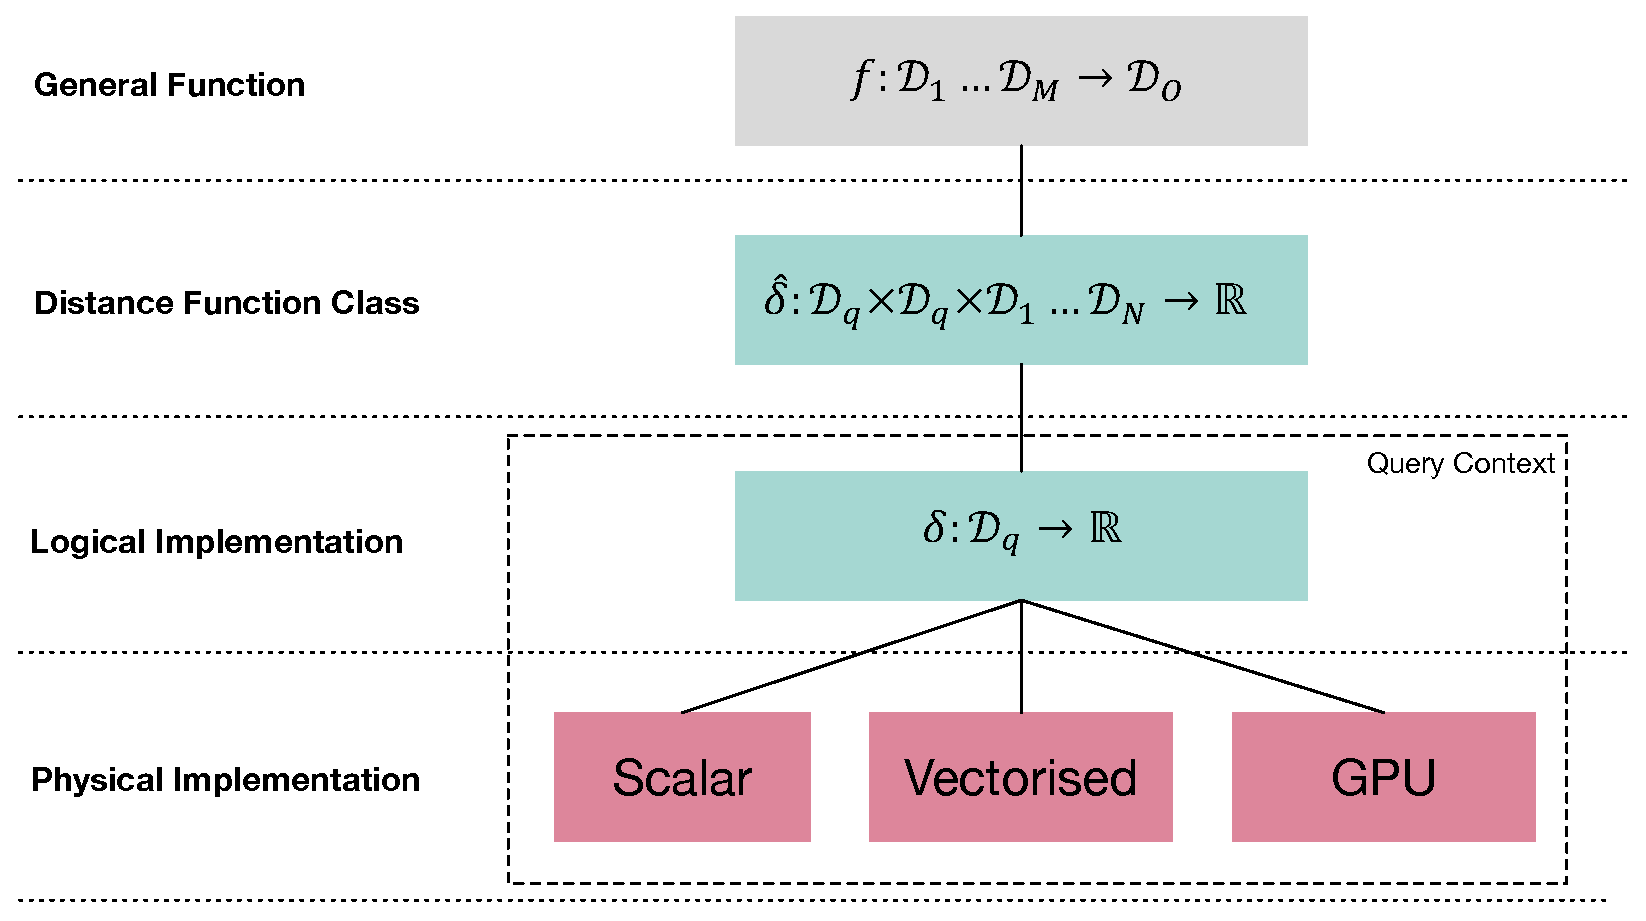
\includegraphics[width=\textwidth]{figures/function_hierarchy.eps}
    \caption{Function hierarchy of all $f \in \mathcal{F}$. As we go down the hierarchy, the \acrshort{dbms} gains knowledge about a function's structure.}
    \label{figure:function_hierarchy}
\end{figure}

\begin{description}
    \item[General Function] Every function $f \in \mathcal{F}$ is known with information about its name and domain (i.e., its signature $\mathtt{SIG}(f)$). This enables the \acrshort{dbms} to provide optimised implementations or replacements for composit operations.
    \item[Distance Function Class] Since DFCs constitute a specific type of function, we can embedd equivalences between a DFC and different types of index structures directly within the function registry. Those equivalences allow a query planner to select one over the other.
    \item[Logical Implementation] As an implementation of a query manifests, the structure of a DFC may change through implementation $\symdist = \mathtt{IMP}(\symdfc)$. For example, certain attributes may turn-out to remain constant, which can be leveraged by the planner to optimise execution.
    \item[Physical Implementation] As the physical execution plan emerges, a plan can make decisions as to what type of implementation for a DFC should be selected. For example, it may select a vectorised version, which leverages \acrshort{simd} instructions of the CPU, over a scalar implementation that calculates the distance in a tight loop.
\end{description}

Optimising implementations of DFCs and general function invocations can be achieved in multiple ways. First, it is reasonable to provide and select implementations that are specific for the data type of the function arguments, so as to avoid type conversion in a tight loop over a large amount of data. This is especially true for \acrshort{dfc}s that operate on complex datatypes, such as vectors. This goes into the direction of \Cref{requirement:complex_data_types}. 

Another aspect that can be optimised is the use of vectorized implementations for computations that involve vectors or matrices, i.e., exchanging a scalar implementation of a \acrshort{dfc} by an implementation that uses \acrshort{simd} instructions. This can be beneficial both for a multimedia \acrshort{dbms} that employs the iteratore model and even more so for a batched processing model. However, for the iterator model it is to expected that one challenge lies in finding the threshold at which usage of such an optimised version pays off. If we take real-valued vectors as an example, it is likely that vectorised execution will not benefit low-dimensional vectors (e.g., $\text{dim} = 3$) while it will greatly benefit high-dimensional vectors (e.g., $\text{dim} = 2048$). Finding this threshold poses challenge in and by itself, which could be subject for future research.

Finally, one can try to match constellations of functions and replace them with an optimised version. A simple example could be the expression $a * b + c$, i.e., $\mathtt{add}(\mathtt{mul}(\mathtt{a},\mathtt{b}), \mathtt{c})$, which can be replaced by a single \emph{fused multiply-add} function $\mathtt{fma}(\mathtt{a},\mathtt{b},\mathtt{c})$ to avoid loss of precission. Replacing the evaluation of a \acrshort{dfc} with a lookup in a high-dimensional index also falls into this category, however, this transformation depends on more than just the function itself.

\subsection{\texorpdfstring{\acrshort{dfc}s}{DFCs} and High-Dimensional Index Structures}

One identity that is particularly relevant for the execution of proximity based queries is the relationship between the execution of a \acrshort{dfc} and the use of a high-dimensional index. As we have discussed in \Cref{section:hd_index_structures}, there exist many different types of indexing techniques that can be used to speed-up \acrshort{nns} in different ways. We propose to formalise the use of high-dimensional indexes\footnote{By ``index'' we refer to a concrete implementation rather than a family since all techniques introduced in \Cref{section:hd_index_structures} can be employed in different ways.} by definining equivalence classes between an index and the relational algebra expressions it replaces. For this, we rely on the index definitions presented in \Cref{section:databases_storage_manager}. In addition to \Cref{definition:index}, the following restrictions may apply in addition to implementation specific restrictions for a specific high-dimensional index: 
\begin{enumerate*}[label=(\roman*)]
    \item High-dimensional indexes are always derived from a feature attribute $\attribute_f \in \schema(\relation)$. Therefore, an index can only replace a DFC if they operate on an unaltered version of $\attribute_f$. Changes to $\attribute_f$, e.g., through application of a nested function $\mathtt{fun}(\attribute_f)$, will render the index unusable unless the same alteration was applied when creating the index.
    \item High-dimensional indexes are sometimes trained for a specific distance function (e.g., Euclidean) or class of distance functions (e.g., Minkowski). Therefore, an index can only replace an expression if the DFC used in that expression coincides with the original function (-class).
\end{enumerate*} Using these constraints, we can now formalise the replacement of a relational expression by an $\mathtt{INDEX}^{\relation}_{I}$ which, for high-dimensional indexes and depending on what expression is matched, falls into one of three classes given by to Definitions \ref{definition:dfc_index_class_1}, \ref{definition:dfc_index_class_2} or \ref{definition:dfc_index_class_3}.

\begin{definition}[label=definition:definition:index_replacement_exact]{Exact Index Replacement}{}
    Let $\relation$ be a relation, $\mathtt{EXP}$ a relational (sub-)expression involving $\relation$ and $\mathtt{INDEX}^{\relation}_{I}$ an index on $\relation$. We call the replacement of $\mathtt{EXP}$ with $\mathtt{INDEX}^{\relation}_{I}$ an \emph{exact index replacement} if $\mathtt{EXP} \equiv \mathtt{INDEX}^{\relation}_{I}$.
\end{definition}

\begin{definition}[label=definition:dfc_index_class_1]{High-Dimensional Index Replacement of Class 1}{}
    Let $\relation$ be a relation, $\attribute_f \in \schema (\relation)$ an attribute of $\relation$ , $\symdfc$ a \acrshort{dfc}, $q \in \domain_f$ a query and $\projection_{P}$ the extended projection involving execution of that \acrshort{dfc} using the query, i.e., $\symdist = \symdfc(\attribute_f, q, \ldots) \in P$. We call a replacement with a high-dimensional index $\mathtt{INDEX}^{\relation}_{\attribute_f, \symdist} \equiv \projection_{\symdist}(\relation)$ \emph{class 1}, if:

    \begin{equation*}
        \projection_{P} (\relation) = \projection_{\symdist}(\relation) \Join_{\mathtt{TID}} \projection_{P \setminus \symdist}(\relation) = \mathtt{INDEX}^{\relation}_{\attribute_f, \symdist} \Join_{\mathtt{TID}} \projection_{P \setminus \symdist}(\relation)
    \end{equation*}
\end{definition}

Class 1 index replacements constitute the simplest and most versatile case but also the least common. The index acts as a drop-in replacement for the distance calculation. While many high-dimensional index-structures in existence can provide this functionality, it rarely makes sense in practice because the speed-up is minimal.

\begin{definition}[label=definition:dfc_index_class_2]{High-Dimensional Index Replacement of Class 2}{}
    Let $\relation$ be a relation, $\attribute_f \in \schema (\relation)$ an attribute of $\relation$ , $\symdfc$ a \acrshort{dfc}, $q \in \domain_f$ a query and $\projection_{P}$ the extended projection involving execution of that \acrshort{dfc} using the query, i.e., $\symdist =\symdfc(\attribute_f, q, \ldots) \in P$ and $\order_{\attribute_{d\updownarrow}}$ be an order operation involving the derived distance attribute $\attribute_{d}$. We call a replacement with a high-dimensional index  $\mathtt{INDEX}^{\relation}_{\attribute_f, \symdfc} \equiv\order_{\attribute_{d\updownarrow}} (\projection_{\symdist}(\relation)) $ \emph{class 2} if:

    \begin{equation*}
        \order_{\attribute_{d\updownarrow}}(\projection_{P} (\relation)) = \order_{\attribute_{d\updownarrow}}(\projection_{\symdist}(\relation)) \Join_{\mathtt{TID}} \projection_{P \setminus \symdist}(\relation) = \mathtt{INDEX}^{\relation}_{\attribute_f, \symdfc} \Join_{\mathtt{TID}} \projection_{P \setminus \symdist}(\relation)
    \end{equation*}
\end{definition}

Class 2 index replacements return a ranked relation that comes pre-sorted according to the derived distance in addition to obtaining the actual distance value. This can be convenient for certain use cases but it is also a rare trait.

\begin{definition}[label=definition:dfc_index_class_3]{High-Dimensional Index Replacement of Class 3}{}
    Let $\relation$ be a relation, $\attribute_f \in \schema (\relation)$ an attribute of $\relation$ , $\symdfc$ a \acrshort{dfc}, $q \in \domain_f$ a query and $\projection_{P}$ the extended projection involving execution of that \acrshort{dfc} using the query, i.e., $\symdist =\symdfc(\attribute_f, q, \ldots) \in P$, $\order_{\attribute_{d\updownarrow}}$ an order operation involving the derived distance attribute $\attribute_{d}$ and $\limit_k$ a $k$-selection. We call a replacement with a high-dimensional index $\mathtt{INDEX}^{\relation}_{\attribute_f, \symdfc} \equiv \limit_k(\order_{\attribute_{d\updownarrow}} (\projection_{\symdist}(\relation)))$ \emph{class 3} if:

    \begin{equation*}
        \limit_k(\order_{\attribute_{d\updownarrow}}(\projection_{P} (\relation))) = \limit_k(\order_{\attribute_{d\updownarrow}}(\projection_{\symdfc}(\relation))) \Join_{\mathtt{TID}} \projection_{P \setminus \symdist}(\relation) =  \mathtt{INDEX}^{\relation}_{\attribute_f, \symdfc} \Join_{\mathtt{TID}} \projection_{P \setminus \symdist }(\relation)
    \end{equation*}
\end{definition}

Class 3 replacements constitute an optimisation of a specific edge-case, which is that of \acrshort{knn} and/or \acrshort{kfn} search. It is probably the most common since it allows for most optimisation but is also the least versatile type of index replacement, since it merely supports one specific type of search. An example of such an index replacement is provided in \Cref{example:index_replacement}

\begin{example}[label=example:index_replacement]{Index Replacement for \acrshort{knn} Search}{}
    The following table lists the schema, extent and rank of $\relation^{\emptyset}_{\mathtt{painting}}$, with their title $\mathcal{A}_{\mathtt{(t)itle}}$, the year of their creation $\mathcal{A}_{\mathtt{(p)ainted}}$ and some arbitrary feature vector $\mathcal{A}_{\mathtt{(f)eature}}$. Let further $\symdfc$ be the Manhattan distance.

    \begin{center}
        \begin{tabular}{ l || l | l | l | l |}
            $\relation^{\emptyset}_{\mathtt{(p)ainting}}$ & $\attributep_{\mathtt{(t)itle}}$  & $\attributef_{\mathtt{(a)rtist}}$ & $\attribute_{\mathtt{(p)ainted}}$ & $\attribute_{\mathtt{(f)eature}}$ \\ 
            \hline
            \hline
            $t_1$ & Mona Lisa &  Leonardo da Vinci & 1506 &  $[2.0,7.0,-8.0]$ \\
            \hline
            $t_2$ & The Starry Night & Vincent van Gogh & 1889 & $[1.0.,0.0,3.0]$ \\
            \hline
            $t_3$ & Las Meninas & Diego Velázquez & 1665 & $[-1.0,3.0,9.0]$ \\
            \hline
            ... & ... & ... & ... & ... \\
            \hline
            $t_N$ & Mars and Venus & Sandro Botticelli & 1483 & $[-3.0,1.0,0.0]$ \\
            \hline
        \end{tabular}
    \end{center}

    The result of the \acrshort{knn}-search
    
    \begin{equation*}
        \relation^{\mathcal{A}_d\uparrow}_{\mathtt{result}} = \lambda_k (\order_{\mathcal{A}_d\uparrow} ( \pi_{\mathcal{A}_{t}, \symdist(\mathcal{A}_{f})} ( \relation_p)))
    \end{equation*}

    can be produced by a class 3 index replacement with $\mathtt{INDEX}^{\relation_{p}}_{\attribute_f, \symdfc}$ and therefore

    \begin{equation*}
        \lambda_k (\order_{\mathcal{A}_d\uparrow} ( \pi_{\mathcal{A}_{t}, \symdist(\mathcal{A}_{f})} ( \relation_p))) = \mathtt{INDEX}^{\relation_{\mathtt{p}}}_{\attribute_f, \symdfc} \Join_{\mathtt{TID}} \projection_{\attribute_{t}} (\relation_p)
    \end{equation*}
    
    A potential index structure could be the \acrshort{vaf} index \cite{Weber:1998Va}.
\end{example}

With the aforementioned definitions and restrictions, we have defined the basic relationship and rules that can be applied by a multimedia \acrshort{dbms}, when deciding whether or not to use a high-dimensional index structure. However, the definitions so far consider the replacement an exact transformation, i.e., the result of the original expression and the index is supposed to be identical. In practice, this is often not the case, which leads to \Cref{definition:index_replacement_inexact} provides an excelent segue to \Cref{section:cost_model}.

\begin{definition}[label=definition:index_replacement_inexact]{Inexact Index Replacement}{}
    Let $\relation$ be a relation, $\mathtt{EXP}$ a relational (sub-)expression involving $\relation$ and $\mathtt{INDEX}^{\relation}_{I}$ an index on $\relation$. We call the replacement of $\mathtt{EXP}$ with $\mathtt{INDEX}^{\relation}_{I}$ an \emph{inexact index replacement} if $\mathtt{EXP} \approx_{b} \mathtt{INDEX}^{\relation}_{I}$ with:
    \begin{equation*}
        \mathtt{EXP} \approx_{b} \mathtt{INDEX}^{\relation}_{I} \leftrightarrow \frac{\mathtt{EXP} \cap \mathtt{INDEX}^{\relation}_{I}}{\mathtt{EXP}} \geq b, b \in [0, 1]
    \end{equation*}
\end{definition}  

\section{Cost Model for Retrieval Accuracy}
\label{section:cost_model}

As we have explained in \Cref{chapter:theory_databases}, most \acrshort{dbms} rely on a cost-model for planning and selecting the execution and access path of a user-specified query. In fact, ever since the System R paper \cite{Selinger:1979Access}, cost-based query planning and optimisation is considered a gold standard for database systems.

Most traditional \acrshort{dbms} exhibit comparatively simple cost-models that mainly rely on the cost incurred by accessing (reading / writing) database pages from or to disk \todo{Source needed?}. Based on what has been discussed thus far, we argue that such a model has several shortcomings and that a cost model for multimedia databases should take the following aspects into account when chosing an execution path:

\begin{description}
    \item[Disk Access (IO)] Persistent storage and the access to information residing on disk is still the factor that contributes the most to long query execution times and is thus something, that a system should try to minimise \cite{Selinger:1979Access}. This is also true for proximity based queries, where part of the optimisation lies in reducing access to vectors.
    \item[CPU] Due to the computational complexity of proximity based operations, especially when high-dimensional vectors are involved, the processing time on CPU is a factor that can no longer be ignored and must thus be taken into account as well. In fact, several index structures achieve speed-up by reducing the computational complexity of the distance calculation \cite{Weber:1998Va,Jegou:2010Product}
    \item[Memory] Some algorithms, e.g., for sorting, can benefit greatly from pure in-memory processing as opposed to writing intermediate results to disk. While memory used to be a scarce resource, some environments allow for complete in-memory processing even for very large datasets.
    \item[Inaccuracy] The inaccuracy of a result incurred, e.g., by the choice of a certain high-dimensional index structure \cite{Indyk1998:Approximate,Jegou:2010Product}, is a price that can be paid to attain speed-up. However, it should be transparent to the system for reasons explained in \Cref{requirement:accuracy_model}.
\end{description}

These four factors can be used to characterise query workloads in a purely local setup consisting of a single node. For distributed databases, obviously, the cost incurred by data and message exchange must be considered as well. However, this is not in scope for the work presented in this Thesis. The aforementioned factors lead us to \Cref{definition:op_cost} and  \Cref{definition:plan_cost} for the (extendable) cost incurred by an operator $\mathtt{OP}$ and query execution plan $\mathcal{P}$.

\begin{definition}[label=definition:op_cost]{Cost of a Relational Operator $\mathtt{OP}$}{}
    Let $\mathtt{OP}$ be a relational operator. The we call the 4-tuple $C_{\mathtt{OP}} = (c_{\mathtt{IO}}, c_{\mathtt{CPU}}, c_{\mathtt{MEM}},c_{\mathtt{ACC}})$ the \emph{cost} of $\mathtt{OP}$, which captures the atomic costs in terms of disk access (IO), CPU usage (CPU), memory usage (MEM) and accuracy (ACC).
\end{definition}

\begin{definition}[label=definition:plan_cost]{Cost of a Query Exection Plan $\mathcal{P}$}{}
    Let $\mathcal{P} = \mathtt{OP}_1 \circ \mathtt{OP}_2, \ldots \circ \mathtt{OP}_N $ be a query execution plan consisting of $N$ operators. The total cost of that plan is given by the sum of the individual costs:

    \begin{equation*}
        C_{\mathcal{P}} = \sum_{i=1}^{N} C_{\mathtt{OP}_i}
    \end{equation*}
\end{definition}

The role of $C_{\mathcal{P}}$ is twofold: First, its absolute values can be used by the \acrshort{dbms} to determine hard constraints imposed for query execution. For example, if there is a fixed limit on memory that can be used by a query, an execution plan may be discarded simply based on exceeding that memory limit regardless of other factors. Similarily, a hard constraint on accuracy could be imposed. Second, it can be used to compare execution plans relatively to one another. \Cref{example:cost_model} illustrates cost calculation for a simple execution plan.

\begin{example}[label=example:cost_model]{Cost of a Query Execution Plan}{}
    Let $\relation_{\mathtt{painting}}$ and $\relation_{\mathtt{artist}}$ be relations from \Cref{example:rel_alg_query}, the query ``return the names of all paintings that were painted by an artist who died after 1800'' results in the following, unoptimised execution plan:

    \begin{equation*}
        \mathcal{P} = \projection_{\attribute_{\mathtt{title}}}(\selection_{\attribute_{\mathtt{death}} > 1800}(\relation_{\mathtt{artist}} \Join \relation_{\mathtt{painting}}))
    \end{equation*}

    This results in the following operator tree with individual and total costs:

    \begin{center}
        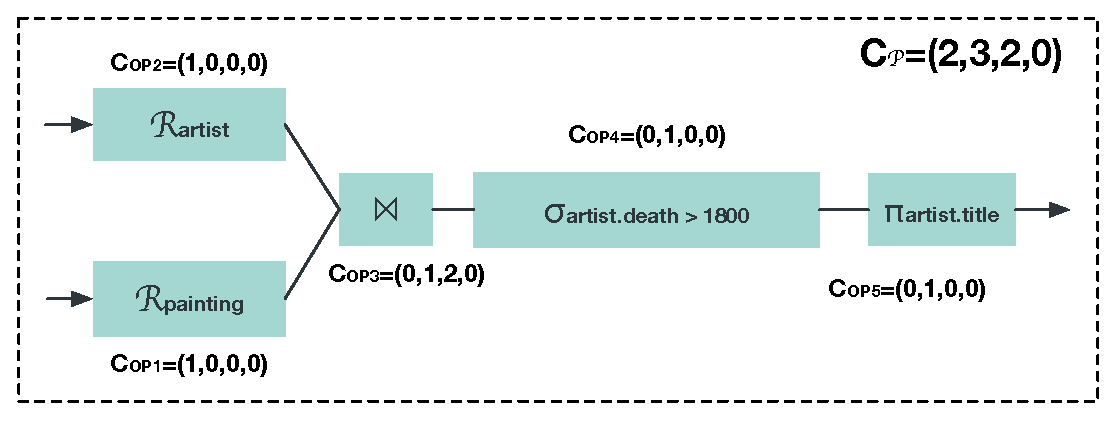
\includegraphics[width=0.9\textwidth]{figures/cost_example.eps}
    \end{center}
\end{example}

The values of the atomic costs per operator can be determined in many ways and the model does not assume any specific approach with the exception for $c_{\mathtt{ACC}}$, which will be described in \Cref{section:inaccuracy_cost_estimation}. However, we do require that the method for determining the atomic costs must be internally consistent and should not change so as to keep costs comparable. For illustrative purposes, we outline the following, rough methods to estimate $c_{\mathtt{IO}}$, $c_{\mathtt{CPU}}$, $c_{\mathtt{MEM}}$.

\begin{description}
    \item[IO Cost Estimation] IO cost can be estimated by estimating the number of pages that must be read / written by an operator. 
    \item[CPU Cost Estimation] CPU cost can be estimated by the number of floating point operations that are executed by an operator (e.g., when executing distance calculations \footnote{Ultimately, this is a property of the \acrshort{dfc} $\symdfc$}).
    \item[Memory Cost Estimation] Memory cost can be estimated by the size of the data structures maintained by an operator (e.g., for sorting or hash-joins).
\end{description}

Since the atomic costs stem from completely different domains and are therefore not directly comparable (e.g., memory costs may be measured in bytes wheras IO costs may be measured in number of page accesses), we require a normalisation step for relative comparison of execution plans. That normalisation step is outline in \Cref{definition:cost_normalisation}.

\begin{definition}[label=definition:cost_normalisation]{Cost Normalisation}{}
    Let $\mathtt{PLANS} = \mathcal{P}_1, \ldots, \mathcal{P}_N$ be $N$ equivalent query execution plans with associated costs $\mathtt{COSTS} =C_{\mathcal{P}_1}, \ldots,C_{\mathcal{P}_N}$. We consider the maximum cost $C_{\mathtt{max}}$ for those plans to be the component-wise maximum of all $C_{\mathcal{P}} \in \mathtt{COSTS}$. Using $C_{\mathtt{max}}$, the normalised cost $ C_{\mathcal{P},i,\mathtt{norm}}$ can be expressed as

    \begin{equation*}
        C_{\mathcal{P},i,\mathtt{norm}} = (\frac{c_{\mathtt{IO},i}}{c_{\mathtt{IO},\mathtt{max}}},\frac{c_{\mathtt{CPU},i}}{c_{\mathtt{CPU},\mathtt{max}}},\frac{c_{\mathtt{MEM},i}}{c_{\mathtt{MEM},\mathtt{max}}},\frac{c_{\mathtt{ACC},i}}{c_{\mathtt{ACC},\mathtt{max}}})
    \end{equation*}

    It follows from the definition, that each component of a normalised cost falls into an interval between $0$ and $1$ due to the normalisation, i.e., $c_{\mathtt{*},\mathtt{norm}} \in [ 0, 1 ]$.
\end{definition}

It is important to note, that the normalised cost can only be used for relative comparison within an existing set of plans. It generally does not provide any information about the original cost value. Using this normalised costs, we can now derive \emph{cost score} according to \Cref{definition:cost_score}.

\begin{definition}[label=definition:cost_score]{Simple Cost Score}{}
    Let $\mathcal{P}$  be a query execution plan with associated, normalised cost $C_{\mathcal{P}_{\mathtt{norm}}}$. We consider the \emph{cost score} to be the sum of the atomic costs.

    \begin{equation*}
        \mathcal{S} = c_{\mathtt{IO},\mathtt{norm}} + c_{\mathtt{CPU},\mathtt{norm}} + c_{\mathtt{MEM},\mathtt{norm}} + c_{\mathtt{ACC},\mathtt{norm}}
    \end{equation*}

    The basic cost score $ \mathcal{S}$ falls into an interval between $0$ and $N$ wherein $N$ denotes the number of atomic costs, i.e., $\mathcal{S} \in [0, $N] for $N = |C_{\mathcal{P}_{\mathtt{norm}}}|$.
\end{definition}

The cost score $\mathcal{S}$ can be used to directly compare query plans and, e.g., sort them in ascending order to select the one plan that minimises the cost.

\subsection{Cost Policies}

The definitions employed so far treat every component of a cost $C_{\mathcal{P}_{\mathtt{norm}}}$ equally with regards to the resulting cost score $\mathcal{S}$. This is rarely desirable since the different component influence the outcome to a different extent (e.g., in terms of query execution time or result accuracy). This can be expressed by employing \emph{cost policy} as outlined in \Cref{definition:cost_policy}.

\begin{definition}[label=definition:cost_policy]{Cost Policy and Weighted Score}{}

    Let $\mathcal{P}$  be a query execution plan with associated, normalised cost $C_{\mathcal{P}_{\mathtt{norm}}}$. We call the 4-tuple

    \begin{equation*}
        \mathcal{W} = (w_{\mathtt{IO}}, w_{\mathtt{CPU}}, w_{\mathtt{MEM}}, w_{\mathtt{ACC}})
    \end{equation*}

    a cost-policy, with $w_{\mathtt{IO}} + w_{\mathtt{CPU}} + w_{\mathtt{MEM}} + w_{\mathtt{ACC}} = 1.0$. The weighted cost score $\mathcal{S}_{\mathcal{W}}$ with respect to $\mathcal{W}$ can be expressed as the linear combination of $C_{\mathcal{P}_{\mathtt{norm}}}$ and $\mathcal{W}$:

    \begin{equation*}
        \mathcal{S}_{\mathcal{W}} = C_{\mathcal{P}_{\mathtt{norm}}} \cdot \mathcal{W} = w_{\mathtt{IO}}c_{\mathtt{IO},\mathtt{norm}} + w_{\mathtt{CPU}} c_{\mathtt{CPU},\mathtt{norm}} + w_{\mathtt{MEM}} c_{\mathtt{MEM},\mathtt{norm}} + w_{\mathtt{ACC}} c_{\mathtt{ACC},\mathtt{norm}}
    \end{equation*}
\end{definition}

The cost policy gives us blunt but simple instrument to assign importance to individual cost factors. For example, we can prioritise execution speed by assigning more weight to the CPU and IO components. In an actual system, $\mathcal{W}$ can be influenced at different levels, which supersede one another, namely 
\begin{enumerate*}[label=(\roman*), itemjoin={{, }}, itemjoin*={{, or, }}, after={{.}}]
    \item as a system-wide configuration
    \item for a user-session (connection-level) or transaction
    \item for an individual query
\end{enumerate*}

\subsection{Estimating Cost of Inaccuracy}
\label{section:inaccuracy_cost_estimation}



\section{Adaptive Index Management}

\begin{figure}[h!]
    \centering
    \begin{subfigure}[b]{0.40\textwidth}
        \centering
        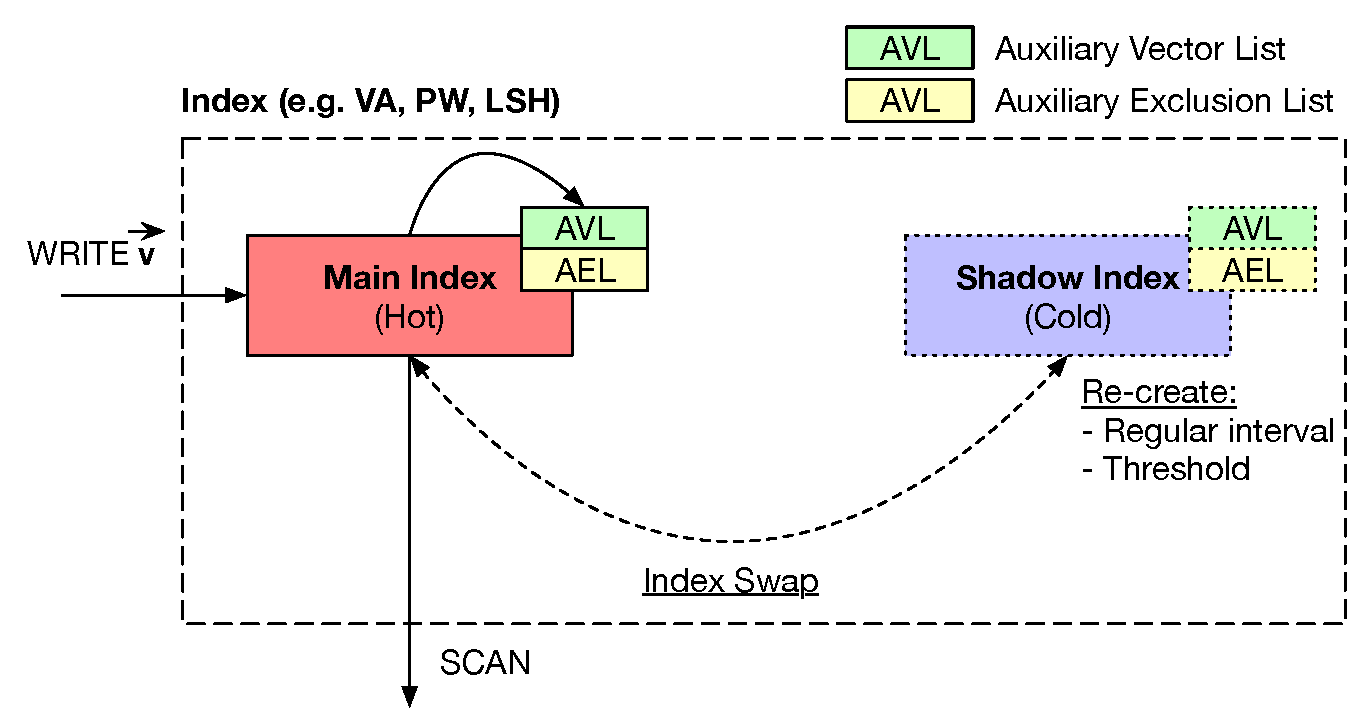
\includegraphics[width=\textwidth]{figures/adaptive_index.eps}
        \label{fig:adaptive_index:architecture}
    \end{subfigure}
    \hfill
    \begin{subfigure}[b]{0.40\textwidth}
        \centering
        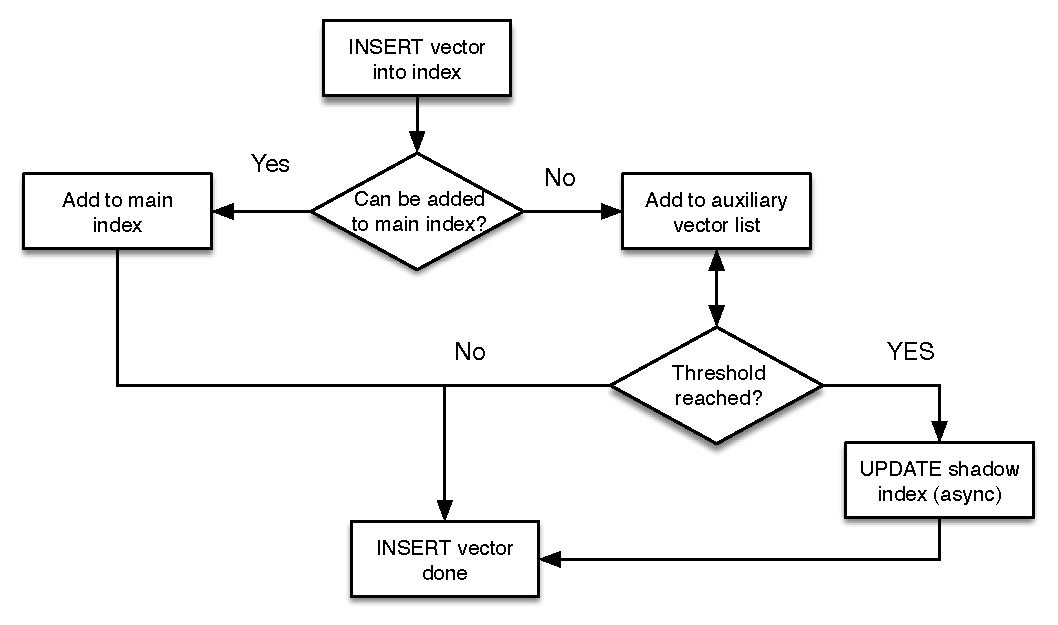
\includegraphics[width=\textwidth]{figures/adaptive_index_flow.eps}
        \label{fig:adaptive_index:flow}
    \end{subfigure}
    \caption{Adaptive index structures overview.}
    \label{fig:adaptive_index}
\end{figure}

Describe model for index management in the face of changing data (adaptive index management):

\begin{itemize}
    \item Reason about properties of secondary indexes for NNS (e.q., PQ, VA, LSH) with regards to data change
    \item Derivation of error bounds possible (e.g., usable for planning)?! Use in query planning?
    \item Systems perspective 1: How to cope with ``dirty'' indexes? Proposal: hot vs. cold index, auxilary data structure, offline optimization, see \cref{fig:adaptive_index}
    \item Systems perspective 2: On-demand index based on query workload?
\end{itemize}

\section{Architecture Model}

\todo[inline]{Putting everything together into a unified systems model (base on previous work + aforementioned aspects).}




